% =====================================================================
% BMED365 (Spring 2027) — Lab 4: Differentiable Neurosymbolic AI Report
% Printable Companion Notebook Export: 05_axiom_stress_tests_and_clinical_translation.ipynb
% Compile with: pdflatex 05_axiom_stress_tests_and_clinical_translation_ipynb.tex (run twice)
% =====================================================================
\documentclass[10pt,a4paper]{article}

\usepackage[utf8]{inputenc}
\usepackage[T1]{fontenc}
\usepackage[english]{babel}
\usepackage{lmodern}
\usepackage{microtype}
\usepackage{graphicx}
\usepackage{booktabs}
\usepackage{xltabular}
\usepackage{tabularx}
\usepackage{array}
\usepackage[table]{xcolor}
\usepackage{amsmath,amssymb,mathtools}
\usepackage{enumitem}
\usepackage[margin=1.7cm,top=1.75cm,bottom=1.85cm,headheight=14pt]{geometry}
\usepackage{fancyhdr}
\usepackage{lastpage}
\usepackage{titlesec}
\usepackage[most]{tcolorbox}
\usepackage{listings}
\usepackage{float}
\usepackage{caption}
\usepackage[hyphens]{url}
\usepackage[
    colorlinks=true,
    linkcolor=uibblue,
    citecolor=uibblue,
    urlcolor=uibred,
    bookmarksnumbered=true,
    bookmarksopen=true,
    pdftitle={05_axiom_stress_tests_and_clinical_translation.ipynb -- Axiom Misspecification and Mass-Effect Stress Tests (BMED365 Spring 2027)},
    pdfauthor={Arvid Lundervold (University of Bergen & MMIV) -- BMED365 Spring 2027},
    pdfsubject={BMED365 Spring 2027 -- Differentiable Neurosymbolic AI Companion Notebook}
]{hyperref}
\def\UrlBreaks{\do\/\do-\do_\do.}
% Allow clean line breaks after underscores in long filenames & Python identifiers
\let\origunderscore\_
\renewcommand{\_}{\origunderscore\allowbreak}

% =====================================================================
% COLORS (UiB / MMIV / BMED365 House Style)
% =====================================================================
\definecolor{uibblue}{RGB}{0, 61, 115}
\definecolor{uibred}{RGB}{175, 28, 44}
\definecolor{kiwigreen}{RGB}{27, 138, 90}
\definecolor{amberwarn}{RGB}{165, 95, 0}
\definecolor{amberbg}{RGB}{255, 250, 240}
\definecolor{lightgray}{RGB}{246, 248, 250}
\definecolor{rowalt}{RGB}{243, 247, 252}
\definecolor{codebg}{RGB}{245, 248, 252}
\definecolor{codehdr}{RGB}{224, 234, 246}
\definecolor{outbg}{RGB}{250, 250, 250}
\definecolor{outhdr}{RGB}{236, 238, 240}
\definecolor{codekw}{RGB}{0, 75, 145}
\definecolor{codestr}{RGB}{155, 35, 45}
\definecolor{codecmt}{RGB}{90, 105, 118}

% =====================================================================
% TYPOGRAPHY, HEADERS & CALLOUT BOXES
% =====================================================================
\setlength{\parindent}{0pt}
\setlength{\parskip}{0.42em}
\setlength{\emergencystretch}{1.8em}
\setlist[itemize]{topsep=2pt,itemsep=2pt,leftmargin=1.45em}
\setlist[enumerate]{topsep=2pt,itemsep=2pt,leftmargin=1.65em}

\newcolumntype{L}[1]{>{\raggedright\arraybackslash}p{#1}}
\newcolumntype{C}[1]{>{\centering\arraybackslash}p{#1}}
\newcolumntype{R}[1]{>{\raggedleft\arraybackslash}p{#1}}
\newcolumntype{Y}{>{\raggedright\arraybackslash}X}

\titleformat{\section}{\large\bfseries\color{uibblue}}{\thesection}{0.65em}{}[\vspace{1pt}\color{uibblue!40}\titlerule]
\titleformat{\subsection}{\normalsize\bfseries\color{uibblue!88!black}}{\thesubsection}{0.55em}{}
\titleformat{\subsubsection}{\small\bfseries\color{uibblue!75!black}}{\thesubsubsection}{0.5em}{}
\titlespacing*{\section}{0pt}{1.05em}{0.4em}
\titlespacing*{\subsection}{0pt}{0.75em}{0.25em}
\titlespacing*{\subsubsection}{0pt}{0.55em}{0.2em}

\pagestyle{fancy}
\fancyhf{}
\fancyhead[L]{\footnotesize\textcolor{gray}{BMED365 (Spring 2027) $\cdot$ Neurosymbolic 7\,T MRI Package}}
\fancyhead[R]{\footnotesize\textcolor{gray}{\texttt{05\_axiom\_stress\_tests\_and\_clinical\_translation.ipynb}}}
\fancyfoot[L]{\footnotesize\textcolor{gray}{University of Bergen \& MMIV $\cdot$ \href{https://github.com/arvidl/BMED365-2027}{\textcolor{gray}{github.com/arvidl/BMED365-2027}}}}
\fancyfoot[R]{\footnotesize\textcolor{gray}{Page \thepage{} of \pageref{LastPage}}}
\renewcommand{\headrulewidth}{0.4pt}
\renewcommand{\footrulewidth}{0.2pt}

\fancypagestyle{firstpage}{
    \fancyhf{}
    \fancyfoot[L]{\footnotesize\textcolor{gray}{University of Bergen \& MMIV $\cdot$ \href{https://github.com/arvidl/BMED365-2027}{\textcolor{gray}{github.com/arvidl/BMED365-2027}}}}
    \fancyfoot[R]{\footnotesize\textcolor{gray}{Page \thepage{} of \pageref{LastPage}}}
    \renewcommand{\headrulewidth}{0pt}
    \renewcommand{\footrulewidth}{0.2pt}
}

% --- Notebook Cell & Pedagogical Boxes ---
\newtcolorbox{seqbox}[1][]{
    enhanced, breakable,
    colback=lightgray, colframe=uibblue,
    colbacktitle=uibblue, coltitle=white,
    fonttitle=\bfseries\small, title={#1},
    boxrule=0.6pt, arc=2.5pt, left=7pt, right=7pt, top=5pt, bottom=5pt
}

\newtcolorbox{codebox}[1][]{
    enhanced, breakable,
    colback=codebg, colframe=uibblue!35,
    colbacktitle=codehdr, coltitle=uibblue!90!black,
    fonttitle=\ttfamily\scriptsize\bfseries, title={#1},
    boxrule=0.55pt, arc=2.2pt, left=6pt, right=6pt, top=3pt, bottom=3pt,
    toptitle=2.5pt, bottomtitle=2.5pt
}

\newtcolorbox{outbox}[1][]{
    enhanced, breakable,
    colback=outbg, colframe=gray!45,
    colbacktitle=outhdr, coltitle=black!75,
    fonttitle=\ttfamily\scriptsize\bfseries, title={#1},
    boxrule=0.5pt, arc=2.2pt, left=6pt, right=6pt, top=3pt, bottom=3pt,
    toptitle=2pt, bottomtitle=2pt
}

\newtcolorbox{clinbox}[1][]{
    enhanced, breakable,
    colback=amberbg, colframe=amberwarn,
    colbacktitle=amberwarn, coltitle=white,
    fonttitle=\bfseries\small, title={#1},
    boxrule=0.6pt, arc=2.5pt, left=7pt, right=7pt, top=5pt, bottom=5pt
}

\newtcolorbox{guidehdr}[1][]{
    enhanced,
    colback=kiwigreen!6, colframe=kiwigreen!75!black,
    borderline west={2.5pt}{0pt}{kiwigreen!85!black},
    boxrule=0.45pt, arc=2pt, left=7pt, right=7pt, top=3.5pt, bottom=3.5pt,
    before skip=0.7em, after skip=0.35em
}

% --- Listings Styles (UTF-8 literate support for pdflatex) ---
\lstdefinestyle{pybmed}{
    language=Python,
    basicstyle=\ttfamily\scriptsize,
    keywordstyle=\bfseries\color{codekw},
    stringstyle=\color{codestr},
    commentstyle=\itshape\color{codecmt},
    showstringspaces=false,
    breaklines=true,
    breakatwhitespace=false,
    breakindent=12pt,
    columns=fullflexible,
    keepspaces=true,
    upquote=true,
    aboveskip=2pt,
    belowskip=2pt,
    xleftmargin=0pt,
    xrightmargin=0pt,
    literate={±}{{$\pm$}}1
             {³}{{\textsuperscript{3}}}1
             {×}{{$\times$}}1
             {é}{{\'e}}1
             {ö}{{\"o}}1
             {Ł}{{\L{}}}1
             {Δ}{{$\Delta$}}1
             {α}{{$\alpha$}}1
             {–}{{--}}1
             {—}{{---}}1
             {≥}{{$\ge$}}1
             {≤}{{$\le$}}1
             {⊂}{{$\subset$}}1
             {∈}{{$\in$}}1
             {→}{{$\to$}}1
             {…}{{\ldots}}1
}

\lstdefinestyle{bashbmed}{
    language=bash,
    basicstyle=\ttfamily\scriptsize,
    keywordstyle=\bfseries\color{codekw},
    stringstyle=\color{codestr},
    commentstyle=\itshape\color{codecmt},
    showstringspaces=false,
    breaklines=true,
    breakatwhitespace=false,
    breakindent=12pt,
    columns=fullflexible,
    keepspaces=true,
    upquote=true,
    aboveskip=2pt,
    belowskip=2pt,
    xleftmargin=0pt,
    xrightmargin=0pt
}

\lstdefinestyle{outbmed}{
    basicstyle=\ttfamily\scriptsize\color{black!85},
    showstringspaces=false,
    breaklines=true,
    breakatwhitespace=false,
    columns=fullflexible,
    keepspaces=true,
    upquote=true,
    aboveskip=1pt,
    belowskip=1pt,
    xleftmargin=0pt,
    xrightmargin=0pt
}

\lstdefinestyle{outbmedwide}{
    basicstyle=\ttfamily\fontsize{6.3pt}{7.6pt}\selectfont\color{black!85},
    showstringspaces=false,
    breaklines=true,
    breakatwhitespace=false,
    columns=fullflexible,
    keepspaces=true,
    upquote=true,
    aboveskip=1pt,
    belowskip=1pt,
    xleftmargin=0pt,
    xrightmargin=0pt
}

\newcommand{\ghblob}{https://github.com/arvidl/BMED365-2027/blob/main}
\newcommand{\colabbase}{https://colab.research.google.com/github/arvidl/BMED365-2027/blob/main}
\newcommand{\repodir}{Lab4-Comp-Imag/Kiwi-challenge/docs/neurosymbolic-report}
\newcommand{\colabbtn}[1]{%
  \href{#1}{\tcbox[on line, arc=2.5pt, boxsep=0pt, left=6pt, right=6pt, top=2.5pt, bottom=2.5pt,
    colback=amberwarn!85!yellow, colframe=white!70!amberwarn, boxrule=0.5pt]{%
    \sffamily\bfseries\scriptsize\color{white}Open in Google Colab}}%
}

% =====================================================================
\begin{document}
\thispagestyle{firstpage}

% --- TITLE BANNER ---
\begin{tcolorbox}[
    enhanced, colback=uibblue, colframe=uibblue,
    arc=3.5pt, left=12pt, right=12pt, top=9pt, bottom=9pt
]
{\Large\bfseries\color{white} Companion Notebook 05 --- Axiom Misspecification \& Pathological Mass-Effect Stress Test\\[2pt]
{\large Soft Bayesian Log-Odds Override vs.\ Rigid Binary Post-Hoc Masking Under Center Shifts \& Organ Scale Mismatch}}\\[4pt]
{\normalsize\color{white!90} BMED365 --- Computational Imaging, Modeling and AI in Biomedicine (Spring 2027)}\\[3pt]
{\footnotesize\color{white!84}
Arvid Lundervold (University of Bergen \& MMIV) $\;\cdot\;$ Reproduces Report Sec.\ 3.5, 4.2, Fig.\ 10 \& Table~9 $\;\cdot\;$ Measured runtime: \texttt{55.4 s} (MPS)
}\\[6pt]
\colabbtn{\colabbase/\repodir/notebooks/05_axiom_stress_tests_and_clinical_translation.ipynb}\hspace{8pt}
{\footnotesize\href{\ghblob/\repodir/notebooks/05_axiom_stress_tests_and_clinical_translation.ipynb}{\textcolor{white}{\underline{\texttt{05\_axiom\_stress\_tests\_and\_clinical\_translation.ipynb} on GitHub}}}}\hspace{10pt}
{\footnotesize\href{\ghblob/\repodir/neurosymbolic-kiwi-report.pdf}{\textcolor{white}{\underline{Technical Report PDF}}}}
\end{tcolorbox}

\begin{seqbox}[Neurosymbolic 7\,T MRI Technical Report --- Companion Package (\texttt{docs/neurosymbolic-report})]
{\footnotesize Companion to \href{\ghblob/\repodir/neurosymbolic-kiwi-report.pdf}{\textbf{\texttt{neurosymbolic-kiwi-report.pdf}}} and shared library \href{\ghblob/\repodir/notebooks/kiwi_ns_lib.py}{\texttt{kiwi\_ns\_lib.py}} (\href{\ghblob/\repodir/notebooks/kiwi_ns_lib_py.pdf}{\textit{annotated PDF}}):}
\begin{enumerate}[start=1, itemsep=1.2pt, topsep=2pt, font=\footnotesize]
    \item \href{\ghblob/\repodir/notebooks/01_data_geometry_and_prior_audit.ipynb}{\texttt{01\_data\_geometry\_and\_prior\_audit.ipynb}} --- 7\,T MRI geometry, empirical audit of Priors 1--3, tri-planar Micro-GT superimposition \& manual GT editing guide (Figs.\ 1--3, Table~3; 27.4\,s MPS).
    \item \href{\ghblob/\repodir/notebooks/02_instancenorm_trap_and_ltn_math.ipynb}{\texttt{02\_instancenorm\_trap\_and\_ltn\_math.ipynb}} --- Experimental proof of \texttt{InstanceNorm3d} coordinate erasure, Bayes Log-Odds \texttt{Organ-GPS}, fuzzy $T$-norms \& LTN $p$-mean autograd sweep (Figs.\ 4--5, Table~4; 7.2\,s MPS).
    \item \href{\ghblob/\repodir/notebooks/03_multiseed_ablation_and_calibration.ipynb}{\texttt{03\_multiseed\_ablation\_and\_calibration.ipynb}} --- 3-seed $\times$ 6-model controlled ablation, operating-point calibration shift \& unmasked whole-organ OOD safety (Figs.\ 6--7, Tables~5--6; 555.1\,s MPS).
    \item \href{\ghblob/\repodir/notebooks/04_mechanistic_interpretability_and_biomarkers.ipynb}{\texttt{04\_mechanistic\_interpretability\_and\_biomarkers.ipynb}} --- Causal neural--symbolic division of labor ($z_{\text{GPS}}$), Mat\'ern hard-core split sweep, error anatomy \& 128-slice NIfTI biomarkers (Figs.\ 8--9, Tables~7--8; 99.3\,s MPS).
    \item \textbf{\texttt{05\_axiom\_stress\_tests\_and\_clinical\_translation.ipynb} (this notebook)} --- Pathological mass-effect center-shift ($\Delta r \in [0, 8]$\,mm) \& radial-scale ($\alpha \in [0.80, 1.25]$) stress tests vs.\ rigid post-hoc masks (Fig.\ 10, Table~9; 55.4\,s MPS).
\end{enumerate}
\end{seqbox}

\subsection*{Purpose}
In clinical medicine, \textbf{pathology frequently breaks textbook anatomy}: a large glioblastoma induces \textbf{midline shift and mass effect}, displacing brain structures by \texttt{5--15 mm} relative to a rigid template! Here we stress-test our trained models under \textbf{synthetic organ center shifts} ($\Delta r \in [0, 8]\text{ mm}$) and \textbf{radial scale errors} ($\alpha \in [0.80, 1.25]$), comparing:
\begin{enumerate}
\item \textbf{Hard Post-Hoc Masking (\texttt{Baseline U-Net $\times$ Rigid Ring Mask})} --- brittle binary symbolic veto.
\item \textbf{Soft Differentiable \texttt{AdditiveBayesOrganNet3D} (\texttt{Rigid-Template Organ-GPS})} --- trained with soft LTN axioms, tested with mismatched coordinates.
\item \textbf{Patient-Adapted \texttt{AdditiveBayesOrganNet3D} (\texttt{Deformable /\allowbreak{} Re-Centered Organ-GPS})} --- the clinical safeguard.
\item \textbf{Unmasked Pure Neural \texttt{Baseline U-Net}} --- locally shift-invariant, yet globally unsafe (\texttt{197k} OOD voxels).
\end{enumerate}

\section*{0. Environment Setup: Portable Execution, Shared Library \& Stress-Test Runtime}
\addcontentsline{toc}{section}{\texorpdfstring{0. Environment Setup: Portable Execution, Shared Library \& Stress-Test Runtime}{0. Environment Setup: Portable Execution, Shared Library and Stress-Test Runtime}}

\begin{guidehdr}
{\small\bfseries\color{kiwigreen!75!black}Conceptual \& Practical Motivation}
\end{guidehdr}
To make the pathological misspecification stress tests directly comparable to Notebooks 03 and 04, this setup cell initializes the exact same shared codebase and cross-platform compute environment:

\begin{itemize}
\item \textbf{Zero-drift shared library (\texttt{kiwi\_ns\_lib.py}):} Imports \texttt{build\_whole\_organ\_geometry()} (supporting synthetic \texttt{center\_shift\_vox} and \texttt{radial\_scale} perturbations), the exact 100-epoch training harness, and \texttt{run\_test\_and\_whole\_fruit()} (supporting \texttt{r\_override} and \texttt{pole\_override} coordinate injection at test time without retraining)---auto-fetched from GitHub \texttt{main} when opened in Colab.
\item \textbf{Runtime device \& output resolution:} \texttt{kns.get\_best\_device()} selects \texttt{CUDA} $\to$ Apple \texttt{MPS} $\to$ \texttt{CPU}, and \texttt{kns.resolve\_report\_dirs()} configures \texttt{FIG\_DIR} and \texttt{RES\_DIR} for saving \textbf{Figure 9} and \texttt{nb05\_stress\_test.json}.
\end{itemize}

\begin{codebox}[{In [1] $\cdot$ Python --- Environment setup, shared library \& coordinate-perturbation runtime}]
\begin{lstlisting}[style=pybmed]
import json
import sys
import urllib.request
from pathlib import Path

# Auto-fetch shared library `kiwi_ns_lib.py` if opened standalone in Google Colab
if not Path("kiwi_ns_lib.py").exists():
    for cand in [Path("docs/neurosymbolic-report/notebooks/kiwi_ns_lib.py"),
                 Path("Lab4-Comp-Imag/Kiwi-challenge/docs/neurosymbolic-report/notebooks/kiwi_ns_lib.py")]:
        if cand.exists():
            sys.path.insert(0, str(cand.parent.resolve()))
            break
    else:
        url = "https://raw.githubusercontent.com/arvidl/BMED365-2027/main/Lab4-Comp-Imag/Kiwi-challenge/docs/neurosymbolic-report/notebooks/kiwi_ns_lib.py"
        print("Downloading kiwi_ns_lib.py from GitHub main for Colab session...")
        urllib.request.urlretrieve(url, "kiwi_ns_lib.py")

if str(Path.cwd()) not in sys.path:
    sys.path.insert(0, str(Path.cwd()))

import importlib.util
for pkg in ("nibabel", "torch"):
    if importlib.util.find_spec(pkg) is None:
        import subprocess
        subprocess.check_call([sys.executable, "-m", "pip", "install", "-q", pkg])

get_ipython().run_line_magic("matplotlib", "inline")
import matplotlib.pyplot as plt
import numpy as np
import pandas as pd
import torch
from scipy import ndimage as ndi
from scipy.spatial.distance import cdist
from skimage import measure

plt.rcParams.update({"figure.dpi": 130, "savefig.dpi": 200, "font.size": 9.5})

import kiwi_ns_lib as kns

DEVICE = kns.get_best_device()
FIG_DIR, RES_DIR = kns.resolve_report_dirs()
print(f"Device: {DEVICE} | Figures -> {FIG_DIR} | Results -> {RES_DIR}")
\end{lstlisting}
\end{codebox}
\begin{outbox}[{Out [1] $\cdot$ stdout}]
\begin{lstlisting}[style=outbmed]
Device: mps | Figures -> <BMED365-2027>/Lab4-Comp-Imag/Kiwi-challenge/docs/neurosymbolic-report/figures | Results -> <BMED365-2027>/Lab4-Comp-Imag/Kiwi-challenge/docs/neurosymbolic-report/results
\end{lstlisting}
\end{outbox}

\section*{1. Run Mass-Effect Center-Shift \& Radial-Scale Misspecification Stress Tests}
\addcontentsline{toc}{section}{\texorpdfstring{1. Run Mass-Effect Center-Shift \& Radial-Scale Misspecification Stress Tests}{1. Run Mass-Effect Center-Shift and Radial-Scale Misspecification Stress Tests}}

\begin{guidehdr}
{\small\bfseries\color{kiwigreen!75!black}Conceptual \& Mathematical Guide: Soft Bayesian Log-Odds Override vs. Brittle Hard Post-Hoc Masking (Table 7 \& Figure 9)}
\end{guidehdr}

\subsubsection*{1.1 The Clinical Critique: What Happens When Pathology Breaks Textbook Anatomy?}
In real clinical MRI, disease frequently distorts normal organ geometry---a glioblastoma causes $5$--$15\,\text{mm}$ of \textbf{midline shift (mass effect)}, ventricular enlargement compresses white matter, and organ atrophy or hypertrophy rescales anatomical radii by $\pm 20\%$--$25\%$. This experiment stress-tests our trained models (without retraining!) under two synthetic coordinate misspecifications produced by \texttt{kns.build\_whole\_organ\_geometry()}:

\begin{enumerate}
\item \textbf{Stress Test 1 --- Mass-Effect Center Shift ($\Delta r \in \{0, 2, 4, 6, 8\}\,\text{mm}$):} Shifts the assumed slice centroid diagonally away from the test wedge by $\Delta x = \Delta y = -\frac{\Delta r / s_x}{\sqrt{2}}$ voxels (so $\|\Delta \mathbf{c}\|_2 = \Delta r$ in physical millimeters), pushing real held-out seeds across the stale compartment boundary:
\[
\tilde{r}_{\text{shift}}(\mathbf{x}) = \frac{\sqrt{\bigl(x - (c_x(z) - \Delta x)\bigr)^2 + \bigl(y - (c_y(z) - \Delta y)\bigr)^2}}{R_{\text{fruit}}(z)}.
\]
\item \textbf{Stress Test 2 --- Radial Scale Mismatch ($\alpha \in \{0.80, 0.90, 1.00, 1.10, 1.25\}$):} Rescales the assumed fruit radius $R'_{\text{fruit}}(z) = \alpha\,R_{\text{fruit}}(z)$, yielding $\tilde{r}_{\text{scale}}(\mathbf{x}) = \tilde{r}(\mathbf{x}) / \alpha$. Setting $\alpha = 0.80$ mimics $-20\%$ atrophy mismatch (expanding $\tilde{r}$ outward past the $0.65$ wall), while $\alpha = 1.25$ mimics $+25\%$ hypertrophy mismatch.
\end{enumerate}

\subsubsection*{1.2 Mathematical Mechanism: Why Soft Bayesian Log-Odds Survives Where Hard Masking Collapses}
Compare how the four regimes combine local MRI appearance with a stale anatomical template $\mathbf{c}^{\text{stale}}(\mathbf{x})$:
\begin{itemize}
\item \textbf{Hard Post-Hoc Binary Masking (\texttt{Baseline U-Net $\times$ Rigid Ring Mask}):} Multiplies predicted probabilities by a rigid binary indicator $\mathbf{1}\{R_{\text{ring}}^{\text{stale}}(\mathbf{x}) \ge 0.5\}$:
\[
p_{\text{hard}}(\mathbf{x}) = p_{\text{base}}(\mathbf{x}) \cdot \mathbf{1}\!\left\{R_{\text{ring}}^{\text{stale}}(\mathbf{x}) \ge 0.5\right\} \quad\Longleftrightarrow\quad \text{log-odds penalty } = -\infty \text{ outside the stale ring!}
\]
No matter how dark and unmistakable a displaced seed is on 7\,T MRI, multiplying by $0$ acts as an unforgiving guillotine---causing a catastrophic cliff at $6\,\text{mm}$ and \textbf{total wipeout ($\text{PQ} = 0.000$) at $8\,\text{mm}$}.
\item \textbf{Soft Differentiable LTN (\texttt{AdditiveBayesOrganNet3D} with mismatched coordinates):} Injects the stale coordinates via \texttt{r\_override} and \texttt{pole\_override} into the finite additive Bayesian log-odds equation:
\[
p_{\text{soft}}(\mathbf{x}) = \sigma\!\Bigl(z_{\text{app}}(\mathbf{X}_3) + z_{\text{GPS}}\bigl(\mathbf{c}^{\text{stale}}(\mathbf{x})\bigr)\Bigr).
\]
Because the learned equatorial wall drop in $z_{\text{GPS}}$ is \textbf{finite} ($\sim -2$ to $-3$ logits), strong local 7\,T $T_2$ visual evidence ($z_{\text{app}} \gg |z_{\text{GPS}}|$) smoothly \textbf{overrides the stale spatial prior} and rescues displaced seeds!
\item \textbf{Patient-Adapted \texttt{Organ-GPS} (Clinical Safeguard):} Computing coordinates deformably from each patient's actual organ contour keeps $\mathbf{c}(\mathbf{x})$ aligned under any shift, locking full peak accuracy ($\text{PQ} = 0.473$).
\item \textbf{Unmasked Pure Neural \texttt{Baseline U-Net}:} Translation-equivariant (constant across $\Delta r$), yet far lower in $\text{PQ}$ ($0.297$) and globally unsafe ($197\text{k}$ OOD voxels).
\end{itemize}

\subsubsection*{1.3 What the Code Below Computes (Table 7 \& Figure 9)}
\begin{enumerate}
\item Trains \texttt{m\_base} and \texttt{m\_ns} (\texttt{100} epochs, seed \texttt{2027}) and locks train-calibrated $\tau_{\text{fg}}^*$.
\item Sweeps both center shifts (\texttt{shifts\_mm}) and radial scales (\texttt{scales}), displays \textbf{Table 7} (\texttt{df\_shift}, \texttt{df\_scale}), and exports \texttt{../\allowbreak{}results/\allowbreak{}nb05\_stress\_test.json}.
\item Renders \textbf{Figure 9}: \textbf{(a)} mass-effect $\text{PQ}$ curves, \textbf{(b)} radial scale mismatch $\text{PQ}$ curves, and \textbf{(c)} a direct mid-slice visual audit at $\Delta r = 6\,\text{mm}$ (\texttt{z = 64}) contrasting the rigid red-dashed mask guillotine against green Soft LTN survival.
\end{enumerate}

\begin{codebox}[{In [2] $\cdot$ Python --- Run mass-effect center-shift ($\Delta r \in [0, 8]$\,mm) \& radial-scale ($\alpha \in [0.80, 1.25]$) stress tests}]
\begin{lstlisting}[style=pybmed]
ds = kns.load_kiwi_dataset()
ssl_bb, _ = kns.pretrain_ssl_backbone(ds, DEVICE, seed=2027, epochs=100)
ubank = kns.sample_unlabeled_blocks(ds, DEVICE, n_blocks=40, seed=2027)

m_base, _, _ = kns.train_neurosymbolic_variant(ds, DEVICE, mode="baseline", epochs=100, seed=2027)
m_ns, _, _ = kns.train_neurosymbolic_variant(
    ds, DEVICE, mode="additive_gps", ssl_backbone=ssl_bb, unlabeled_bank=ubank,
    p_quant=3.0, w_comp=2.0, w_t2=1.2, gps_lr=1.5e-2, epochs=100, seed=2027,
)
thr_cal = kns.calibrate_threshold_on_train(m_ns, "additive_gps", ds, DEVICE, use_split=True)

# Precompute baseline U-Net test probabilities once (purely local texture -> invariant to coordinate shifts)
res_base_unmasked = kns.run_test_and_whole_fruit(m_base, "baseline", ds, DEVICE, thresh=0.50, use_split=False, do_whole_fruit=False)
res_ns_adapted = kns.run_test_and_whole_fruit(m_ns, "additive_gps", ds, DEVICE, thresh=thr_cal, use_split=True, do_whole_fruit=False)

# Stress Test 1: Synthetic organ center displacement (0 .. 8 mm, simulating clinical mass-effect / midline shift!)
shifts_mm = [0.0, 2.0, 4.0, 6.0, 8.0]
shift_rows = []
demo_4mm = {}

for s_mm in shifts_mm:
    # Shift organ center diagonally away from the test sector (+x, +y -> shifts true seeds toward inner/outer walls!)
    dv = (s_mm / ds.spacing[0]) / np.sqrt(2.0)
    _, r_sh, z_sh, ring_sh = kns.build_whole_organ_geometry(ds.vol, ds.spacing, center_shift_vox=(-dv, -dv, 0.0), radial_scale=1.0)
    pole_sh = (np.abs(z_sh - 0.5) * 2.0).astype(np.float32)

    # 1. Hard Post-Hoc Binary Ring Mask on Baseline U-Net
    ring_te = ring_sh[ds.rx0:ds.rx1, ds.ry0 + ds.split_y : ds.ry1, ds.rz0:ds.rz1] >= 0.50
    lbl_hard = kns.decode_deep_watershed_3d((res_base_unmasked["prob_te"] >= 0.50) & ring_te, res_base_unmasked["dist_te"], ds.spacing)
    ev_hard = kns.evaluate_semantic_and_instance_3d(lbl_hard, ds.test_gt)

    # 2. Soft Differentiable LTN with Rigid (Mismatched) Coordinates
    res_soft = kns.run_test_and_whole_fruit(
        m_ns, "additive_gps", ds, DEVICE, thresh=thr_cal, use_split=True,
        r_override=r_sh, pole_override=pole_sh, do_whole_fruit=False,
    )
    ev_soft = res_soft["ev_te"]

    if abs(s_mm - 6.0) < 1e-6:
        demo_4mm = {"ring_te": ring_te, "lbl_hard": lbl_hard, "lbl_soft": res_soft["pred_te"], "ev_hard": ev_hard, "ev_soft": ev_soft}

    shift_rows.append({
        "shift_mm": s_mm,
        "hard_mask_PQ": ev_hard["PQ"], "hard_mask_Rec": ev_hard["Recall"], "hard_mask_Pred": ev_hard["Pred"],
        "soft_ltn_PQ": ev_soft["PQ"],  "soft_ltn_Rec": ev_soft["Recall"],  "soft_ltn_Pred": ev_soft["Pred"],
        "adapted_ltn_PQ": res_ns_adapted["ev_te"]["PQ"],
        "unmasked_base_PQ": res_base_unmasked["ev_te"]["PQ"],
    })

df_shift = pd.DataFrame(shift_rows)
display(df_shift)

# Stress Test 2: Radial Organ Scale Mismatch (alpha in [0.80 .. 1.25], simulating organ hypertrophy / atrophy)
scales = [0.80, 0.90, 1.00, 1.10, 1.25]
scale_rows = []
for sc in scales:
    _, r_sc, z_sc, ring_sc = kns.build_whole_organ_geometry(ds.vol, ds.spacing, radial_scale=sc)
    pole_sc = (np.abs(z_sc - 0.5) * 2.0).astype(np.float32)
    ring_te = ring_sc[ds.rx0:ds.rx1, ds.ry0 + ds.split_y : ds.ry1, ds.rz0:ds.rz1] >= 0.50
    ev_h = kns.evaluate_semantic_and_instance_3d(
        kns.decode_deep_watershed_3d((res_base_unmasked["prob_te"] >= 0.50) & ring_te, res_base_unmasked["dist_te"], ds.spacing),
        ds.test_gt,
    )
    ev_s = kns.run_test_and_whole_fruit(
        m_ns, "additive_gps", ds, DEVICE, thresh=thr_cal, use_split=True,
        r_override=r_sc, pole_override=pole_sc, do_whole_fruit=False,
    )["ev_te"]
    scale_rows.append({
        "radial_scale": sc,
        "hard_mask_PQ": ev_h["PQ"], "hard_mask_Rec": ev_h["Recall"],
        "soft_ltn_PQ": ev_s["PQ"],  "soft_ltn_Rec": ev_s["Recall"],
    })

df_scale = pd.DataFrame(scale_rows)
display(df_scale)

(RES_DIR / "nb05_stress_test.json").write_text(json.dumps({"center_shift": shift_rows, "radial_scale": scale_rows}, indent=2), encoding="utf-8")

# Figure 9: 3-Panel Axiom Misspecification & Mass-Effect Stress Test
fig, axes = plt.subplots(1, 3, figsize=(16.0, 4.0))

axes[0].plot(df_shift["shift_mm"], df_shift["adapted_ltn_PQ"], "k--", lw=1.6, label="Patient-Adapted Organ-GPS (safeguard)")
axes[0].plot(df_shift["shift_mm"], df_shift["soft_ltn_PQ"], "o-", color="#1b8a5a", lw=2.3, label="Soft Differentiable LTN (graceful decay)")
axes[0].plot(df_shift["shift_mm"], df_shift["hard_mask_PQ"], "s-", color="#e74c3c", lw=2.3, label="Hard Post-Hoc Binary Mask (brittle cliff!)")
axes[0].axhline(res_base_unmasked["ev_te"]["PQ"], color="#7f8c8d", ls=":", lw=1.5, label="Unmasked Baseline U-Net (globally unsafe)")
axes[0].set_xlabel("Simulated Organ Center Shift / Mass Effect Δr (mm)")
axes[0].set_ylabel("Held-Out 3D Panoptic Quality (PQ)")
axes[0].set_title("(a) Mass-Effect Center-Shift Stress Test\nSoft LTN resists moderate shift; hard mask collapses!")
axes[0].legend(fontsize=7.2, loc="lower left")
axes[0].grid(alpha=0.25)

axes[1].plot(df_scale["radial_scale"], df_scale["soft_ltn_PQ"], "o-", color="#1b8a5a", lw=2.3, label="Soft Differentiable LTN")
axes[1].plot(df_scale["radial_scale"], df_scale["hard_mask_PQ"], "s-", color="#e74c3c", lw=2.3, label="Hard Post-Hoc Binary Mask")
axes[1].axvline(1.00, color="k", ls=":", lw=1.2, label="True Organ Scale (1.00)")
axes[1].set_xlabel("Radial Atlas Scale Mismatch Factor α")
axes[1].set_ylabel("Held-Out 3D Panoptic Quality (PQ)")
axes[1].set_title("(b) Organ Size / Hypertrophy Mismatch\nSoft log-odds survives where binary veto fails")
axes[1].legend(fontsize=7.5, loc="lower center")
axes[1].grid(alpha=0.25)

# Panel (c): Visual comparison at 6 mm mass-effect shift on mid-test slice z=64
zm = 8
te_vn = ds.vol_norm[ds.rx0:ds.rx1, ds.ry0 + ds.split_y : ds.ry1, ds.rz0:ds.rz1]
axes[2].imshow(te_vn[:, :, zm].T, cmap="gray", origin="lower")
axes[2].contour(ds.test_gt[:, :, zm].T > 0, levels=[0.5], colors=["#f1c40f"], linewidths=1.2)
axes[2].contour(demo_4mm["ring_te"][:, :, zm].T, levels=[0.5], colors=["#e74c3c"], linewidths=1.6, linestyles="--")
soft_fg = demo_4mm["lbl_soft"][:, :, zm].T > 0
axes[2].imshow(np.ma.masked_where(~soft_fg, soft_fg), cmap="Greens", alpha=0.55, origin="lower", vmin=0, vmax=1.2)
axes[2].set_title(f"(c) 6 mm Shift Audit (z=64): Yellow=GT\nRed dashed=hard mask (PQ={demo_4mm['ev_hard']['PQ']:.2f}) | Green=Soft LTN ({demo_4mm['ev_soft']['PQ']:.2f})")
axes[2].axis("off")

plt.tight_layout()
fig.savefig(FIG_DIR / "fig09_mass_effect_stress_test.png", bbox_inches="tight")
plt.show()
\end{lstlisting}
\end{codebox}
\begin{outbox}[{Out [2a] $\cdot$ DataFrame --- Stress Test 1: Synthetic Organ Center Shift / Mass Effect ($\Delta r \in [0, 8]$\,mm)}]
\centering
{\scriptsize
\setlength{\tabcolsep}{3.6pt}
\renewcommand{\arraystretch}{1.18}
\rowcolors{2}{rowalt}{white}
\begin{tabular}{r r r r r r r r r}
\toprule
\rowcolor{uibblue!12}\textbf{$\Delta r$ (mm)} & \textbf{Hard PQ} & \textbf{Hard Rec} & \textbf{Hard Pred} & \textbf{Soft PQ} & \textbf{Soft Rec} & \textbf{Soft Pred} & \textbf{Adapt.\ PQ} & \textbf{Base PQ} \\
\midrule
0.0 & 0.3267 & 0.5769 & 57 & 0.4734 & 0.5385 & 32 & 0.4734 & 0.2968 \\
2.0 & 0.3282 & 0.5769 & 51 & 0.4617 & 0.5192 & 31 & 0.4734 & 0.2968 \\
4.0 & 0.2293 & 0.3462 & 31 & 0.4621 & 0.5192 & 30 & 0.4734 & 0.2968 \\
\textbf{6.0} & \textbf{0.0896} & \textbf{0.1154} & \textbf{13} & \textbf{0.4524} & \textbf{0.5192} & \textbf{30} & \textbf{0.4734} & \textbf{0.2968} \\
\textbf{8.0} & \textbf{0.0000} & \textbf{0.0000} & \textbf{2} & \textbf{0.4328} & \textbf{0.5192} & \textbf{30} & \textbf{0.4734} & \textbf{0.2968} \\
\bottomrule
\end{tabular}
}
\end{outbox}
\begin{outbox}[{Out [2b] $\cdot$ DataFrame --- Stress Test 2: Radial Organ Scale Mismatch ($\alpha \in [0.80, 1.25]$)}]
\centering
{\scriptsize
\setlength{\tabcolsep}{3.6pt}
\renewcommand{\arraystretch}{1.18}
\rowcolors{2}{rowalt}{white}
\begin{tabular}{r r r r r}
\toprule
\rowcolor{uibblue!12}\textbf{Scale $\alpha$} & \textbf{Hard Mask PQ} & \textbf{Hard Mask Rec} & \textbf{Soft LTN PQ} & \textbf{Soft LTN Rec} \\
\midrule
\textbf{0.80} & \textbf{0.2394} & \textbf{0.3654} & \textbf{0.4598} & \textbf{0.5192} \\
0.90 & 0.3397 & 0.5769 & 0.4606 & 0.5192 \\
\textbf{1.00} & \textbf{0.3267} & \textbf{0.5769} & \textbf{0.4734} & \textbf{0.5385} \\
1.10 & 0.3070 & 0.5769 & 0.4710 & 0.5385 \\
1.25 & 0.2993 & 0.5769 & 0.4625 & 0.5385 \\
\bottomrule
\end{tabular}
}
\end{outbox}
\begin{figure}[H]
    \centering
    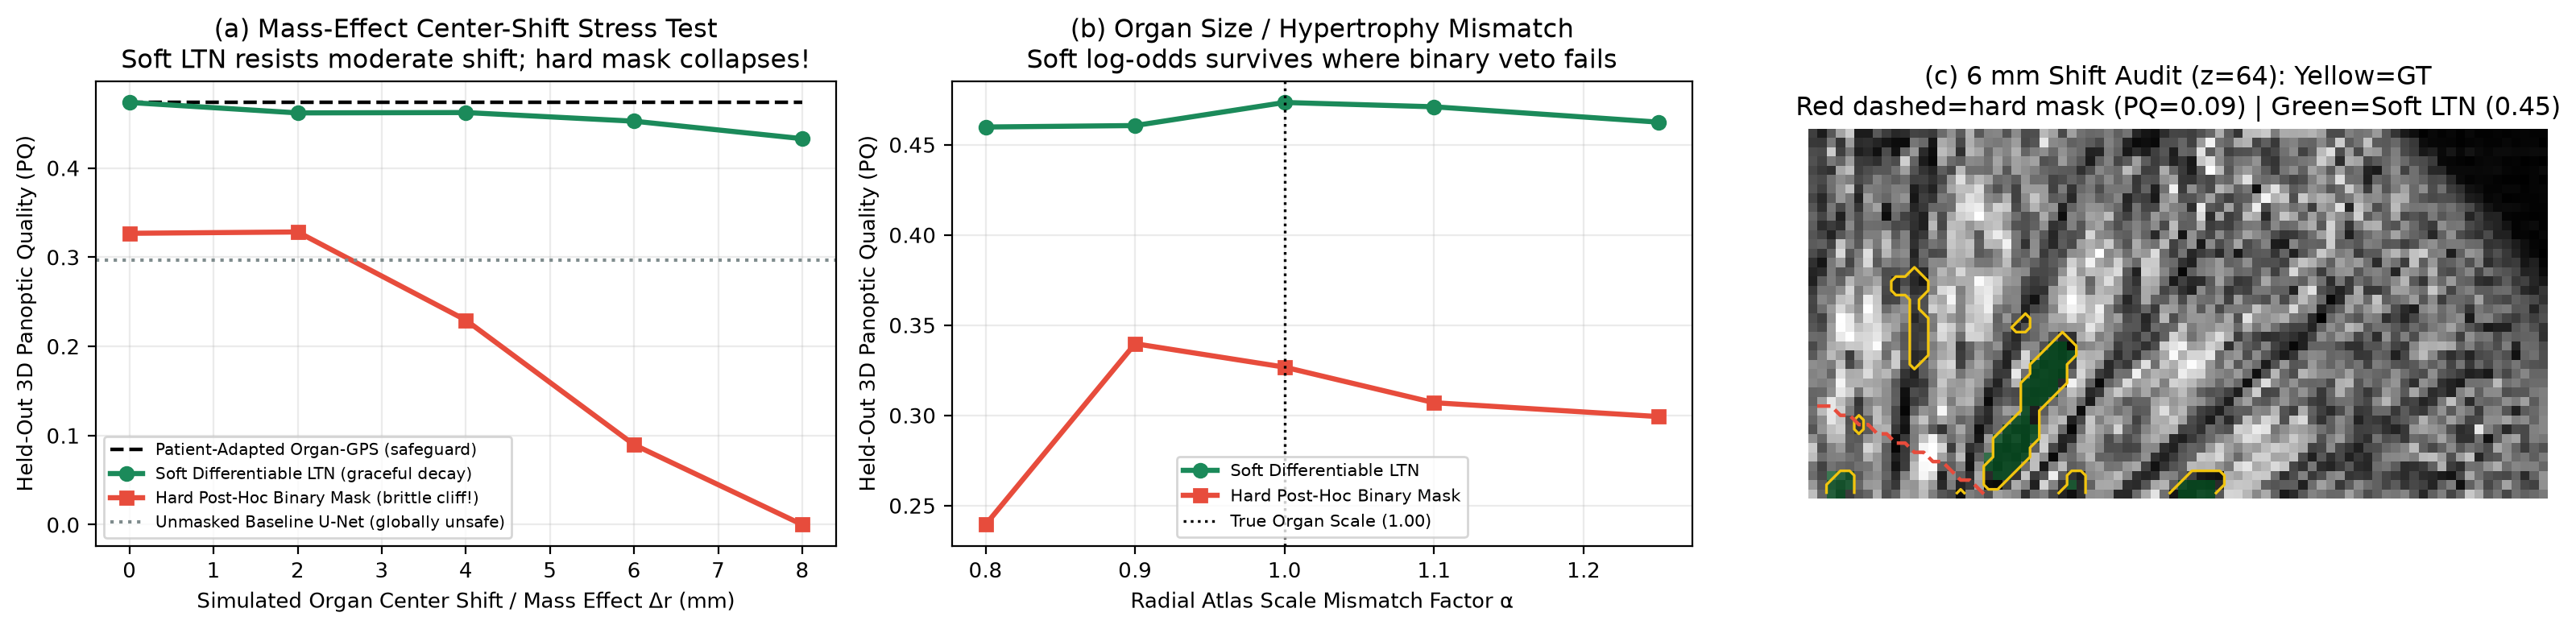
\includegraphics[width=\textwidth]{../figures/fig09_mass_effect_stress_test.png}
    \vspace{-4pt}
    \caption*{\footnotesize\textit{Executed Figure~9 / Report Figure~10 (\texttt{Out [2]}, saved as \texttt{fig09\_mass\_effect\_stress\_test.png}): (a)~Center-shift mass-effect stress test ($\Delta r = 0$--$8\,\text{mm}$) contrasting Soft Differentiable LTN graceful survival ($\text{PQ} = 0.433$ at $8\,\text{mm}$) against hard binary mask wipeout ($\text{PQ} = 0.000$); (b)~radial scale mismatch ($\alpha \in [0.80, 1.25]$); (c)~mid-slice visual audit at $\Delta r = 6\,\text{mm}$ ($z = 64$).}}
\end{figure}

\end{document}
